\documentclass[tikz,border=12pt]{standalone}
\usepackage{tikz}
\usetikzlibrary{arrows.meta}

\begin{document}

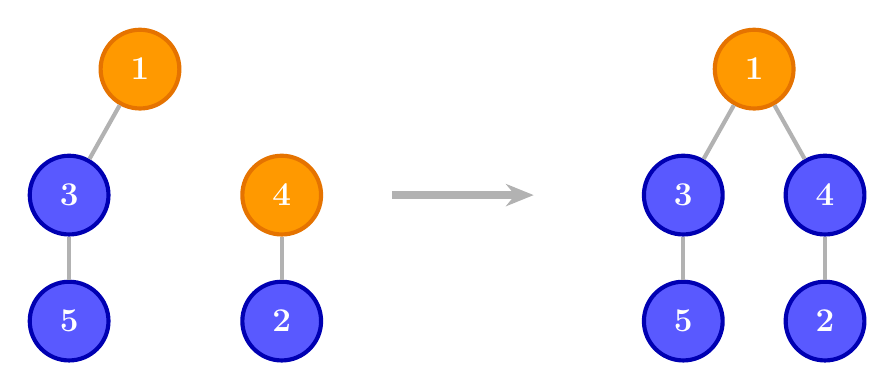
\begin{tikzpicture}[
  yellownode/.style={circle, draw=orange!90!black, fill=orange!80!yellow,
                     text=white, font=\bfseries\large, minimum size=1cm, line width=1.5pt},
  bluenode/.style={circle, draw=blue!70!black, fill=blue!65,
                   text=white, font=\bfseries\large, minimum size=1cm, line width=1.5pt},
  edge/.style={draw=gray!60, line width=1.5pt},
]

% ── Left: Tree 1 (root = 1) ────────────────────────────────────────────
\node[yellownode] (1L) at (0,    0)    {1};
\node[bluenode]   (3L) at (-0.9, -1.6) {3};
\node[bluenode]   (5L) at (-0.9, -3.2) {5};

\draw[edge] (1L) -- (3L);
\draw[edge] (3L) -- (5L);

% ── Left: Tree 2 (root = 4, separate) ─────────────────────────────────
\node[yellownode] (4L) at (1.8,  -1.6) {4};
\node[bluenode]   (2L) at (1.8,  -3.2) {2};

\draw[edge] (4L) -- (2L);

% ── Arrow ──────────────────────────────────────────────────────────────
\draw[->, gray!60, line width=3pt, -{Stealth[length=10pt,width=8pt]}]
  (3.2, -1.6) -- (5.0, -1.6);

% ── Right: Merged tree (root = 1) ─────────────────────────────────────
\node[yellownode] (1R) at (7.8,  0)    {1};
\node[bluenode]   (3R) at (6.9, -1.6)  {3};
\node[bluenode]   (5R) at (6.9, -3.2)  {5};
\node[bluenode]   (4R) at (8.7, -1.6)  {4};
\node[bluenode]   (2R) at (8.7, -3.2)  {2};

\draw[edge] (1R) -- (3R);
\draw[edge] (3R) -- (5R);
\draw[edge] (1R) -- (4R);
\draw[edge] (4R) -- (2R);

\end{tikzpicture}

\end{document}
